\documentclass[a4paper]{report}
\usepackage{a4wide}
\usepackage[utf8]{inputenc}
\usepackage[T1]{fontenc}
\usepackage{parskip}
\usepackage{hyperref}
\usepackage{epsfig}
\usepackage{background}
\usepackage{mathptmx}

% To avoid tikz error, see https://tex.stackexchange.com/questions/165929/semiverbatim-with-tikz-in-beamer
\makeatletter
\global\let\tikz@ensure@dollar@catcode=\relax
\makeatother

\backgroundsetup{
scale=1,
angle=0,
opacity=1,
contents={
\includegraphics[width=\paperwidth,height=\paperheight]{images/spi-front.jpg}}
}

\hypersetup{
  colorlinks   = true,
  urlcolor     = blue,
  linkcolor    = blue,
  pdfinfo = {
    Title = {SPI Annual Report 2022},
    Author = {Software in the Public Interest, Inc.},
    Keywords = {SPI, free software, open source, FOSS, annual report, charity, non-profit, 501c3},
  }
}

\begin{document}

\title{Software in the Public Interest, Inc.\\
2022 Annual Report}
\date{July 10, 2023}

\maketitle

\newpage

\backgroundsetup{
scale=1,
angle=0,
opacity=1,
contents={
\includegraphics[width=\paperwidth,height=\paperheight]{images/spi-content.jpg}}
}

\hspace{1em}

To the membership, board and friends of Software in the Public Interest, Inc:

As mandated by Article 8 of the SPI Bylaws, I respectfully submit this annual report on the activities of Software in the Public Interest, Inc. and extend my thanks to all of those who contributed to the mission of SPI in the past year.

  \emph{-- Michael Schultheiss, SPI President}

\newpage

\tableofcontents

\newpage

\chapter{Committee Reports}
\section{Membership Committee}

\subsection{Statistics}

On January 1, 2022 we had 243 contributing and 1253 non-contributing members.  On December 31, 2022 there were 258 contributing members and 1299 non-contributing members.  This is an increase of 15 contributing members and an increase of 46 non-contributing members.

\chapter{Board Report}
\section{Board Members}

Board members as of January 1, 2022:

\begin{itemize}
\item Michael Schultheiss (President)
\item Stephen Frost (Vice President)
\item Tim Potter (Secretary)
\item Héctor Orón Martínez (Treasurer)
\item Joe Conway
\item Forrest Fleming
\item Milan Kupcevic
\item Chris Lamb
\item Martin Zobel-Helas
\end{itemize}

Board members as of December 31, 2022:

\begin{itemize}
\item Michael Schultheiss (President)
\item Stephen Frost (Vice President)
\item Forrest Fleming (Secretary)
\item Héctor Orón Martínez (Treasurer)
\item Joe Conway
\item Milan Kupcevic
\item Jonatas L. Nogueira
\item Jeremy Stanley
\item Zach van Rijn
\end{itemize}

\section{Board Changes}

Changes that occurred during the year:

\begin{itemize}

\item The terms for Forrest Fleming, Chris Lamb, Héctor Orón Martínez, and Martin Zobel-Helas expired in July 2022.  Tim Potter stepped down from the board.  Forrest and Héctor sought, and obtained, re-election.  We'd like to thank Chris, Martin and Tim for their work on the board.  Jonatas L. Nogueira, Jeremy Stanley, and Zach van Rijn joined the board as part of the same election.

\item On August 8, 2022 the board voted to appoint the following officers:

\begin{itemize}
\item President: Michael Schultheiss
\item Vice President: Stephen Frost
\item Secretary: Forrest Fleming
\item Treasurer: Héctor Orón Martínez
\end{itemize}

\end{itemize}

\section{Elections}

A board membership election was conducted in July 2022.  There were 5 board seats up for election.  Nominations were received from Forrest Fleming, Jonatas L. Nogueira, Héctor Orón Martínez, Zach van Rijn, and Jeremy Stanley.  Since there were 5 nominations for 5 board seats, no vote was required and all three candidates were elected for a 3 year term.

\chapter{Treasurer's Report}

SPI will publish audited financial statements later in July or August.

\chapter{Member Project Reports}

\section{New Associated Projects}

\subsection{Battle for Wesnoth}

\href{https://www.wesnoth.org/}{Battle for Wesnoth} is an open source, turn-based strategy game with a high fantasy theme. It features both single-player and online/hotseat multiplayer combat. The game also allows its users to create their own ``campaigns'' and make them publicly available, as well as collaborating with the core team to expand the open source gaming ecosystem.

\subsection{MPI Forum}

The \href{https://www.mpi-forum.org/}{MPI Forum} is the standardization body for the Message Passing Interface (MPI), a hardware agnostic interface for passing messages for parallel and distributed computing. MPI is implemented in a number of open-source and proprietary libraries and widely used in academic, corporate, and research institutions. The MPI Forum meets regularly to discuss and design the next version of the MPI Standard. The work of the MPI Forum happens in our public GitHub repositories, and anyone is welcome to participate by joining the MPI Forum's mailing list and attending our virtual and physical meetings.

\section{Projects No Longer Associated with SPI}

\begin{itemize}

\item Chakra Linux is no longer active.

\item Glucosio is no longer active.

\end{itemize}

\section{Updates from Associated Projects}

\subsection{0 A.D.}

\href{https://play0ad.com/}{0 A.D.} (pronounced ``zero ey-dee'') is a cross-platform, real-time strategy (RTS) game of ancient warfare. It is a historically-based war/economy game, in which the player must lead an ancient civilization, gather resources, and raise a military force to conquer enemy factions. 0 A.D. is open source software licensed under the GPL, and its art and sound assets are licensed under CC BY-SA. It is developed by Wildfire Games, a global community of game developers.

In 2022, the Han (Chinese) faction was added to 0 A.D. in the 26th release expanding our "reach" to the far east. Along with it came twenty-six new music tracks for people to enjoy, improved art and the usual balance changes. Players can now also play on two new maps: one set in the Tarim Basin in northwestern China, and another, set around the Yangtze River. To improve the user interface, we included icons on the minimap for special
structures.

Team members also presented the game at FOSS community events including Play Sorbonne U, the Stunfest, the Japan Tours Festival, the Vandoeuvre in Game, the Capitole du Libre, and DevCon \#16. These outreach efforts helped raise awareness of 0 A.D. and facilitated recruitment of contributors.

We wish to extend our thanks to our generous donors and to SPI for helping us achieve this progress.

{\em Submitted by Aviv Sharon}

\subsection{Adélie Linux}

\href{https://www.adelielinux.org/}{Adélie} is a lightweight, musl-based, independent Linux platform for desktop and server use, committed to integrity, privacy, and user freedom.

The Adélie Linux distribution continued to deliver on its commitments. In 2022, we fixed over 500 issues that could affect the performance, security, integrity, or user experience of our platform.

While we were not able to reach our third release candidate, RC3, in 2022 an additional 1100 updates by 11 contributors brought a modern, rock-solid desktop experience to our users. Highlights include up-to-date Perl, Python, LLVM, Rust, Linux kernel, and desktop environments.

We're excited to announce a new collaboration with the \href{https://gw4.ac.uk/news/new-strategic-partnership-launched-between-gw4-alliance-and-the-western-gateway/}{GW4 Alliance} (a partnership between U.K.-based universities, Cray Inc., and the U.K. Met Office) for access to an ARM-based Cray XC50 production supercomputer called Isambard, clocking in at 20,992 cores.

Adélie is on track to target supercomputers after the 1.0 general release. We now include Spack, a package manager for supercomputers, giving users access to thousands of scientific software packages and bringing us closer to our goal of making Adélie into a musl-based platform for high-performance computing (HPC).

Our future is bright. Thank you to our \href{https://git.adelielinux.org/groups/adelie/-/group_members}{team}, our \href{https://www.adelielinux.org/sponsors/}{sponsors}, and our users for being part of it. Follow our \href{https://blog.adelielinux.org/}{blog} and \href{https://www.adelielinux.org/contact/}{social media accounts} to stay informed about our progress!

{\em Submitted by Zach van Rijn}

\subsection{Ankur.org.in}

During the past year, members of the project have met a few times in person and virtually to deliberate on the focus and direction of our energies. We sensed that the original gap around creating tools and infrastructure to enable content localization is no longer the most crucial topic. However, what is important is to engage with content producers, including independent content producers covering socially relevant issues. In most instances, the highest audience engagement is when the content is in English and yet this creates a content gap for the audience, which is more comfortable engaging in Bengali.

To test this hypothesis, the members have been conducting workshops
with independent media rooms and individual content publishers to introduce them to the glossary of technical terms and content translation methods that produce reasonably high-quality content. This year, we have focused more on written content since automatic content translation tools are available to speed things up. There have been six workshops in 2022, with a few more planned in the first half of 2023. We are still working on a plan for engaging with video content creators, especially video bloggers.

Our ongoing challenge is that members have been busy in their day jobs, and with the current economic and employment situation as it is -- we see that as an emergent threat to the sustainability of this effort.

{\em Submitted by Sankarshan Mukhopadhyay}

\subsection{Arch Linux}

\href{https://archlinux.org/}{Arch Linux} is a lightweight and flexible Linux distribution that tries to Keep It Simple. In 2022, the Arch Linux project made significant advancements in technology and community outreach.

To streamline contributions, we migrated several of our projects to our \href{https://gitlab.archlinux.org}{gitlab.archlinux.org GitLab}, allowing for more efficient collaboration. In addition, we enhanced community outreach efforts by starting to publish documentation, accepted RFCs, and \href{https://monthly-reports.archlinux.page/}{monthly reports} to our new archlinux.page domain.

One notable improvement is the introduction of creating debug packages by default as well as hosting a {\tt debuginfod} service. This service facilitates easier debugging by providing source listings and debug symbols to users utilizing debuggers like {\tt gdb} and {\tt delve}, benefiting both packagers and users who analyze and debug issues or crashes.

We also fundamentally reworked our keyring tooling, which manages trust in our official package distribution. To address the challenges posed by PGP keyserver reliability, we now store relevant data in-tree and generate our Web Key Directory
(WKD) data automatically from our GitLab repository.

Another significant achievement is the progress made toward migrating from SVN to Git for package sources. Core projects such as {\tt dbscripts} and {\tt devtools} have first proof of concept versions ready for testing, paving the way for a future switch.

Furthermore, we modernized the backend of our AUR platform, leveraging Python and the Starlette/FastAPI framework.

{\em Submitted by Levente Polyák}

\subsection{ArduPilot}

\href{https://ardupilot.org/}{ArduPilot} is a cross-platform free software autopilot project for a wide range of robotic vehicles. ArduPilot continues to thrive, with our global and growing community of users, partners and developers continuing to achieve remarkable things.The 2022 Developers Conference was again a virtual event, and was a great success --- the flexibility and additional participation provided by online attendance adds significant value and will be continued into the future. (2023 will be a hybrid event hosted in Canberra, Australia.)

Our Partners Program continues to grow, again enabling and requiring additional staff for managing the quantity and quality of code contributions, and provide real-time support to industry. The direct engagement with commercial users of ArduPilot provided by the Partners Program helps advance the project beyond simply financial support, and it is exciting to see it evolve.  The ArduPilot Foundation, a Not-For-Profit incorporated in Australia with the express purpose of supporting the ArduPilot project, is now in it's second year, and has proven an excellent complement to the support provided by SPI.

{\em Submitted by James Pattison}

\subsection{Battle for Wesnoth}

The \href{https://www.wesnoth.org/}{Battle for Wesnoth} is a cross-platform turn based strategy game. It features both single player and online/hotseat multiplayer content, both as part of the main game as well as an expansive modding system that allows players to create and share their own creations. Battle for Wesnoth is open source software with its code and textual elements licensed under the GPL v2+ while art, music, and sounds are licensed under a mix of GPL v2+ and CC BY-SA.

In 2022, fixes continued to be made to Wesnoth's current stable release (1.16). In the development releases (1.17), a new campaign was added exploring the early history of one of the default factions which did not previously have a dedicated campaign. A variety of new units were added, primarily monster and various fauna, as well as new terrains including the ability to have terrain visually appear higher or lower than the surrounding hexes. Graphical performance has also been significantly improved by moving to using SDL's hardware accelerated rendering as opposed to software rendering.

{\em Submitted by Pentarctagon}

\subsection{Debian}

During 2022, \href{https://www.debian.org/}{Debian} voted to include non-free firmware in our default images for the Debian 12 (bookworm) release.  This has become necessary on most consumer hardware for even basic networking and display features to function. We'll continue to work on enabling Debian for free hardware, and provide more images to accommodate such hardware in the future.

We also released four point releases for Debian 11, and two point releases for Debian 10, which incorporates security updates and critical fixes for these stable releases.

We gained 19 new Debian Developers, and 34 new Debian Maintainers who we hope will also become full project members in the future.

To stay up to date with what's happening in the Debian project, subscribe to the \href{https://bits.debian.org/}{Bits from Debian website}.

{\em Submitted by Jonathan Carter}

\subsection{FFmpeg}

\href{https://www.ffmpeg.org/}{FFmpeg} is a complete, cross-platform solution to record, convert and stream audio and video. It is used as the foundation platform of many projects dealing with multimedia, both open source and proprietary, and is used extensively by several web-based multimedia conversion and processing services.

In the year 2022, FFmpeg delivered the 5.0 major release in January, the 5.1 point release in July as well as many security updates of old releases.  A complete list of changes can be found in \href{https://git.ffmpeg.org/gitweb/ffmpeg.git/blob/HEAD:/Changelog}{the changelog}.

FFmpeg joined the GSoC 2022 program again, successfully completing two student projects.  After the pandemic crisis, we had a developer meeting in December 2022 again and are preparing for more meetings and conferences for the next year.

{\em Submitted by Submitted by Thilo Borgmann}

\subsection{LibreOffice}

In 2022, The Document Foundation (TDF) released two major versions of \href{https://www.libreoffice.org/}{LibreOffice}, starting with LibreOffice 7.3 in February. This release included major improvements to change tracking, along with Bash-like auto-completion for AutoInput in Calc. Later in the year, LibreOffice 7.4 introduced WebP support, new typographical settings for hyphenation, and support for 16,384 columns in spreadsheets.

Throughout 2022, TDF and the LibreOffice community organised events and supported free software campaigns around the world. The LibreOffice Conference 2022 took place in-person again (after two online events due to the pandemic), in Milan, northern Italy. There were also two ``Month of LibreOffice'' campaigns, which encouraged LibreOffice users to also become contributors.

{\em Submitted by Mike Saunders}

\subsection{ns-3}

\href{https://www.nsnam.org}{ns-3} is a discrete-event, packet-level network simulator with an emphasis on networking research and education.

In 2022, ns-3 published two software releases of the main simulator, thanks to submissions from thirty-nine contributors.  Software engineering was a major focus for the development team; the project replaced the build system, Python bindings framework, continuous integration system, and the base coding style.  Improvements were made to the modeling capability for the current Wi-Fi 6 standard, to the propagation models for 4G/5G cellular simulations, and to several models for wireless personal area networks.  ns-3 also mentored two student projects in the 2022 edition of Google Summer of Code, and organized its fourteenth annual academic workshop, featuring seventeen technical paper presentations and several lightning talks and tutorial sessions. The workshop was held online due to the pandemic.

{\em Submitted by Tom Henderson}

\subsection{Open Bioinformatics Foundation}

The \href{https://www.open-bio.org/}{Open Bioinformatics Foundation} (OBF), founded in 2001, is a non-profit, volunteer-run group that promotes open source development and open science in biological research. OBF is led by an elected Board that currently includes \href{https://open-bio.org/board/}{9 members}, with Peter Cock as the president. In the past year, one Board member, Malvika Sharan, finished her term. Iddo Friedberg (Iowa State University) was elected on 2022-10-21 as a new member-at-large.  Board member Nomi Harris was elected as Secretary, replacing Chris Fields in that role.

In 2022, OBF awarded 19 Event Fellowships as part of its program to increase diverse participation at events that promote open science. OBF participated in Google Summer of Code 2022, with five students, all from underrepresented groups, working on open source bioinformatics-related projects.

OBF's annual Bioinformatics Open Source Conference, BOSC 2022, was part of ISMB 2022 (in Madison, WI, and online – the first hybrid ISMB). Keynote speaker Jason Williams gave a BOSC / Education COSI keynote entitled ``Riding the bicycle: Including all scientists on a path to excellence''. A joint session with Bio-Ontologies featured a keynote by Melissa Haendel, ``The open data highway: turbo-boosting translational traffic with ontologies''. The program also included a panel discussion on ``Building and Sustaining Inclusive Open Science Communities'', with panelists who not only are known for supporting diversity and inclusion, but also themselves are members of groups that are underrepresented in our field.

{\em Submitted by Nomi Harris}

\subsection{OpenSAF}

\href{https://opensaf.sourceforge.io/}{OpenSAF} is a high availability middleware, which helps in achieving 99.999\% of service availability to business and mission critical applications. It is the fastest and the most efficient middleware implementation of AIS specifications from SA Forum. OpenSAF is being used mostly in telecom and defence applications worldwide. OpenSAF can detect fault and perform recovery in few milliseconds.

In 2022, we made significant contributions to OpenSAF. We delivered 3 major releases:

\begin{itemize}

\item \href{https://sourceforge.net/p/opensaf/wiki/NEWS-5.22.01/}{OpenSAF-5.22.01}
\item \href{https://sourceforge.net/p/opensaf/wiki/NEWS-5.22.06/}{OpenSAF-5.22.06}
\item \href{https://sourceforge.net/p/opensaf/wiki/NEWS-5.22.11/}{OpenSAF-5.22.11}

\end{itemize}

{\em Submitted by Nagendra Kumar}

\subsection{OpenZFS}

\href{https://openzfs.org/}{OpenZFS} held its annual Developer Summit in October 2022, returning to an in-person event. The event was a little smaller than in the past, but we had 11 presentations from people at 9 companies and one independent member of the community. There were 55 attendees in person at the event, over a hundred concurrent viewers of the live stream, and thousands of views of the recordings.

The main technical work in 2022 was BLAKE3 checksum support, and Block Reference Tracking, which will be part of the upcoming OpenZFS 2.2 release.  We also published 5 patch releases with bug fixes and small features.

{\em Submitted by Matthew Ahrens}

\subsection{PostgreSQL}

\href{https://www.postgresql.org/}{PostgreSQL} is a powerful, open-source relational database management system that emphasizes extensibility, robustness, and SQL compliance.

In 2022 we released PostgreSQL 15 as the latest major version of our core database server software. This new release includes several important improvements and features for database users. One of the most notable is the improved compression and sorting performance, which can lead to significant speed-ups in certain workloads.

Additionally, this release includes new expressive developer features, such as the SQL standard MERGE command, new regular expression functions, and the ability to create views that query data using the permissions of the caller. PostgreSQL 15 also provides more options for managing logical replication, simplifying conflict management, and adding support for two-phase commit (2PC) with logical replication.  Other notable changes include a new logging format, {\tt jsonlog}, and the ability for users to manage PostgreSQL configuration parameters.

The PostgreSQL community also saw a return to pre-pandemic levels with over two dozen in-person community conferences and events around the world. Through our non-profit work we were also able to expand our contributor appreciation activities as well as continue outreach work via our Google Summer of Code participation, which included mentorship projects involving 12 students this year (up from 7 a year ago). With the end of the pandemic we have also started to see a return of local meetup participation and have been coordinating with volunteers within the community to learn how we can support them.

{\em Submitted by Robert Treat}

\subsection{Privoxy}

In 2022 \href{https://www.privoxy.org/}{Privoxy} development continued but no new release was published.

{\em Submitted by Fabian Keil}

\subsection{systemd}

systemd is a suite of basic building blocks for a Linux system. It provides a system and service manager that runs as PID 1 and starts the rest of the system.

In 2022 we published two major releases of systemd and 44 point releases with bug fixes. We merged 5428 commits (down from 5968 in 2021) from a total of 364 contributors. We organized a \href{https://lpc.events/event/16/sessions/146/#20220912}{micro-conference at Linux Plumbers} in September, and we participated in the \href{https://uapi-group.org/docs/minutes/2022-10-05__image-based-linux-summit/}{Image-Based Linux Summit in Berlin in October}. We continue to hold a biweekly maintainers meeting and the project is maintaining a steady pace of development.

{\em Submitted by Luca Boccassi}

\subsection{The Mana World}

\href{https://www.themanaworld.org/about}{The Mana World} (TMW) is an organisation that, starting in 2004 from a single game, has over the years spawned several development projects aiming to create innovative free and open source MMORPGs (massively multiplayer online role-playing games) based around the unique TMW art style and a shared wealth of assets that are used to build different gaming experiences. TMW currently offers two playable titles and one ambitious overhaul project in its early stages.

{\em The Mana World: Classic} is the original game that has been in constant development for almost 20 years. On TMW Classic you will find a world of quests, exploration and many years of accumulated content. The game currently hosts the majority of our longstanding community. Due to the game's age, its development is slowed by an outdated engine, which is the main reason why developers have sought to branch out with adjacent projects featuring engine improvements.

Our second game is {\em Moubootaur Legends}, a game constantly growing, developed with a special emphasis on feedback from players. New features are added as players request them and the aim is to provide a faster turnaround that allows us to create a large playable world in less time. The game allows you to explore a wide range of assets that have been built for different TMW projects all in one world, thus providing hours of gameplay. This is at the expense of some bugs and inconsistent themes, but the game is still much beloved for the quantity of content it provides.

{\em Source of Mana} is our newest project, born in 2022. It aims to create a consistent and high-quality MMORPG that re-captures the essence of The Mana World in a completely new engine built on Godot. The game is in its very early stages of development and most of the work is currently focused on building the foundations of the new engine.

Over the past year, The Mana World has undergone significant changes, formalising it as a publisher organisation of multiple independent projects including but not limited to its original game. Existing projects have been centralised under the TMW umbrella in order to allow for better cooperation and to let everyone benefit from our modest but established brand. Development efforts are mostly focused on our dedicated game client, {\em Moubootaur Legends} and {\em Source of Mana}.

{\em Submitted by The Mana World development team}

\subsection{Translatewiki.net}

\href{https://translatewiki.net/}{Translatewiki.net} is an online translation platform for free and open source projects and volunteer translators. Our activity has been stable at around 1,600 active yearly translators making around 550k translations.

On the development side, we added new features to increase collaboration between translators. With an experimental terminology tool translators can add translations for common terms and expressions. Those translations are shown in the translation interface. We are also showing edit summaries
directly in the translation interface so that it's easier to see when and why translation has been changed.

Towards the end of the year our mail relay was shut down and we had to learn how to set up our own mail delivery system on a short notice.  Additionally, we improved our deployment tooling so that it is possible to test configuration changes in production before deploying.

{\em Submitted by Niklas Laxström}

\subsection{Tux4Kids}

The \href{https://tuxpaint.org/}{Tux Paint} project celebrated its 20th birthday in June 2022, with a new release that added a paint-style color mixer, improvements to the color picker, a brush spacing option for the paint and line tools, and other updates.

Ahead of the new release, a 3-part historical retrospective of the project was posted on the project's website.  The site's new art gallery also continued to grow, and we were excited to see a band's music video created using a combination of Tux Paint and Blender.

{\em Submitted by Bill Kendrick}


\appendix
\chapter{About SPI}

SPI is a non-profit organization which was founded to help organizations develop and distribute open hardware and software. We encourage programmers to use the GNU General Public License or other licenses that allow free redistribution and use of software, and hardware developers to distribute documentation that will allow device drivers to be written for their product.

SPI was incorporated as a non-profit organization on June 16, 1997 in the state of New York. Since then, it has become an umbrella organization for projects from the community.

In 1999, the Internal Revenue Service (IRS) of the United States government determined that under section 501(a) of the Internal Revenue Code SPI qualifies for 501(c)(3) (non-profit organization) status under section 509(a)(1) and 170(b)(1)(A)(vi). This means that donations made to SPI and its supported projects are tax-deductible as charitable donations for US taxpayers.

\newpage

\pagestyle{empty}

\backgroundsetup{
scale=1,
angle=0,
opacity=1,
contents={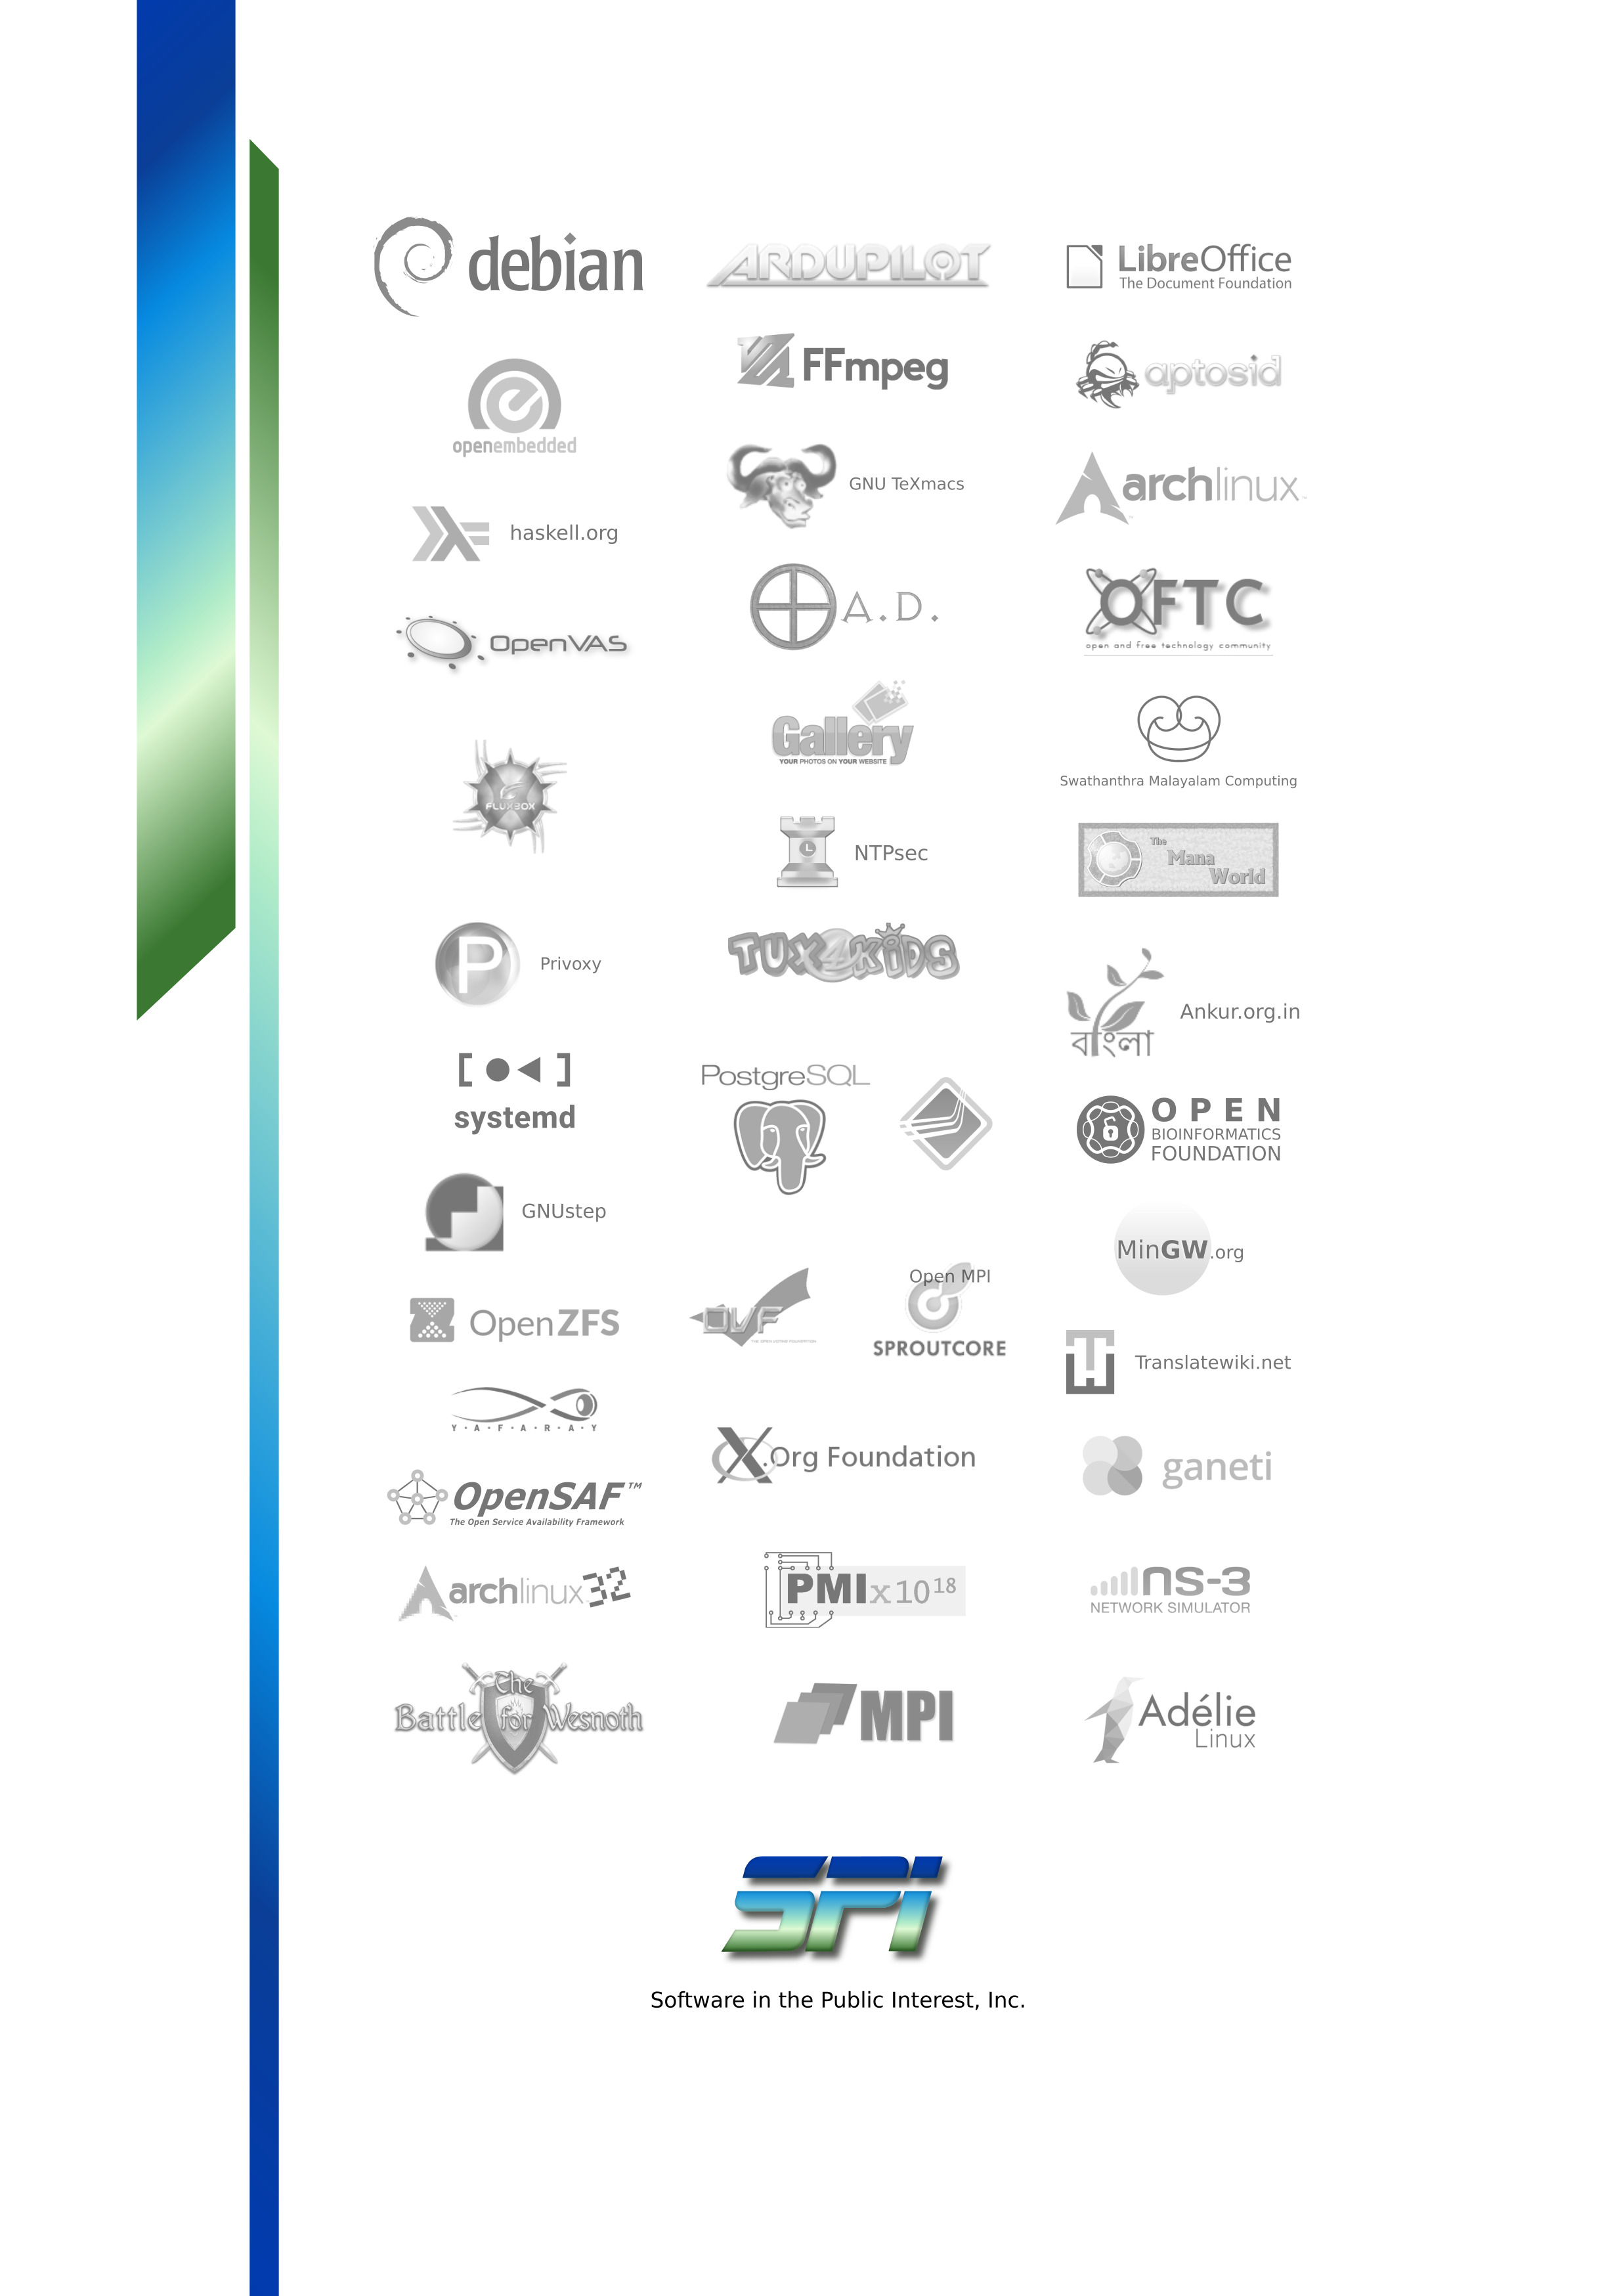
\includegraphics[width=\paperwidth,height=\paperheight]{images/spi-back-2022.jpg}}
}

\null

\end{document}
% Keep this at the bottom, thanks.
% Local Variables:
% TeX-master: "report"
% End:
